\section{Material und Methoden}
\label{sec:durchführung}
%Rahmenbedinungen der Untersuchung
%Auswahl, Einschränkungen und Begründungen
%Erhebungs-, Mess- und Auswertungsverfahren
%Womit und wie haben Sie untersucht ?

\subsection{Ist-Analyse}
\subsubsection{Aktuelles Dosierverfahren}
\subsubsection{Produktionsweise}
\subsection{Rechnerische Auslegung}
\subsubsection{Berechnung des Druckverlustes für verschiedene Leitungsdurchmesser}
\subsubsection{Rohrleitungsklassifizierung nach PAS 1057}
\subsection{Fachgespräche und Angebotsanfragen}

\subsection{Experimentelle Untersuchungen}
\subsubsection{Ermittlung der Viskosität nach DIN EN ISO 2555}
Eine Möglichkeit die dynamische Viskosität einer Dispersion zu bestimmen, ist die Messung mit einem Rotationsviskosimeter nach DIN EN ISO 2555. Da in dieser Norm hauptsächlich ein Rotationsviskosimeter mit Einzelzylinder beschrieben ist, wird an dieser Stelle auf die DIN ISO 3219 verwiesen. In dieser Norm werden zusätzlich Rotationsviskosimeter mit koaxialem Zylinder und Kegel-Platte-Viskosimeter näher beschrieben. \cite{DINDeutschesInstitutfurNormunge.V..Februar2013, DINDeutschesInstitutfurNormunge.V..September2018} \\

Das bei \textsc{Alberdingk Boley Leuna GmbH} verwendete Verfahren zur Viskositätsbestimmung ist angelehnt an die DIN EN ISO 2555 unter Nutzung eines digitalen \textsc{Brookfield}-Rotationsviskosimeters, benannt nach dem Hersteller \textsc{AMETEK$^\text{\textregistered}$\,Brookfield}. Diese Viskosimeter haben den Vorteil preisgünstig zu sein und erlauben ein Messen der Viskosität direkt im Probengefäß. Da jedoch durch das direkte Eintauchen in ein theoretisch beliebiges Probengefäß nur eingeschränkte Übertragbarkeiten und Reproduzierbarkeiten möglich sind, können diese Geräte hauptsächlich für Vergleichsmessungen genutzt werden.  Der Hersteller gibt hierfür an ein \SI{600}{\milli \liter} Becherglas als Probengefäß zu nutzen, jedoch wird in der DIN\,EN\,ISO\,2555 darauf hingewiesen, dass die Becherglasgröße freigewählt werden darf. Für den Vergleich von Messungen rät die Norm dennoch jeweils die gleiche Größe des Becherglases zu nutzen. \cite{ROMPPRedaktion.2008, brookfield_31.01.2022, DINDeutschesInstitutfurNormunge.V..September2018}

\begin{wrapfigure}{R}{0.33\textwidth}
	\centering
	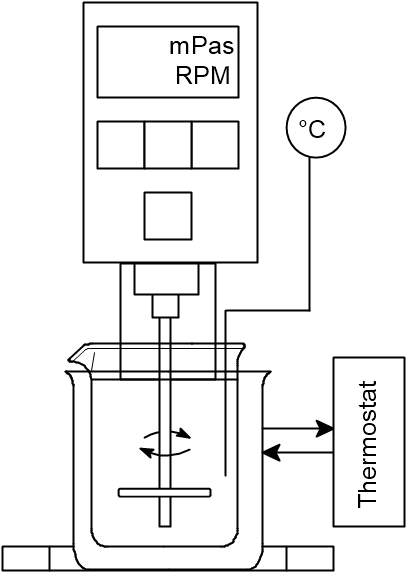
\includegraphics[width=0.25\textwidth]{img/viskosimeter}
	\caption{Viskositätsmessung mit digitalem \textsc{Brookfield}-\linebreak Rotationsviskosimeter}
	\label{fig: viskosimeter}
\end{wrapfigure}
\FloatBarrier
%Ende

Die Messung mittels digitalem \textsc{Brookfield}-Viskosimeter ist vergleichsweise einfach. Benötigt werden hierfür das Viskosimeter in einer Halterung, ein Becherglas, ein Temperaturmessgerät und eine herstellerspezifische Spindel. Soll die Viskosität bei bestimmten Temperaturen, abweichend der Labortemperatur bestimmt werden, ist zusätzlich ein thermostatisches Flüssigkeitsbad nötig (vgl. Abb. \ref{fig: viskosimeter}). \newpage 
Die Messung lässt sich nach dem Aufbau über das Bedienfeld starten in dem Spindel und Drehzahl eingegeben werden. Sobald die Messung startet beginnt sich die Spindel zu drehen.\\
Das Messprinzip eines solchen \textsc{Brookfield}- \linebreak Viskosimeters basiert auf der Messung der Winkelabweichung, auch Torsion genannt, zwischen der im Viskosimeter verbauten Welle und einer zweiten darunter angeordneten Spindel-Welle mit fest definierten geometrischen Körper. Beide Wellen drehen sich dabei mit der selben Drehzahl  und sind über eine Federeinheit verbunden. Bei Digital-Viskosimetern wird der Messwert der sich dann durch die Winkelabweichung ergibt direkt über ein Display angezeigt.\\
Entscheidend für die Messung der Viskosität ist bei dieser Messmethode die Auswahl des bereits erwähnten Becherglases, sowie der Spindel und der Drehzahl. Spindel und Drehzahl werden dabei unter Einbezug des Viskositätbereiches der Probe nach der gewünschten Präzision und dem Geschwindigkeitgefälle ausgewählt. \cite{DINDeutschesInstitutfurNormunge.V..September2018} 
Durch Tabellen des Herstellers, welche sowohl Spindel als auch Viskositätsbereich in Abhängigkeit von Drehzahl und Gerätekonstanten berechnen lassen, werden diese Entscheidungen vereinfacht. \cite{brookfield_31.01.2022} 

\subsubsection{Erwärmungsverhalten}
\subsubsection{Verdünnungsverhalten}
\subsubsection{Pumpversuche}

\subsection{Nutzwertanalyse}

\subsubsection{Erarbeitung von Lösungsvarianten}
\subsubsection{Festlegen und gewichten von Entscheidungskriterien}
\subsubsection{Bewertung der Lösungsvarianten}
\subsubsection{Gesamtbeurteilung der Varianten}

\subsection{Computerunterstützes Zeichnen von Plänen}
\subsubsection{Software: AutoCAD}

\subsection{Gefährdungsbeurteilung (HAZOP-Verfahren)}


